% !TEX TS-program = XeLaTeX
% use the following command: 
% all document files must be coded in UTF-8
\documentclass[spanish]{textolivre}
% See more information on the repository: https://github.com/leolca/textolivre

% Metadata
\begin{filecontents*}[overwrite]{article.xmpdata}
    \Title{Fidelidad y praxeologías en aplicaciones didácticas desarrolladas para la resolución de expresiones matemáticas}
    \Author{Alberto Camacho Ríos \sep Bertha Ivonne Sánchez Luján \sep Marisela Caldera-Franco}
    \Language{es}
    \Keywords{Praxeología \sep Fidelidad \sep app.m.}
    \Journaltitle{Texto Livre}
    \Journalnumber{1983-3652}
    \Volume{14}
    \Issue{3}
    \Firstpage{1}
    \Lastpage{11}
    \Doi{10.35699/1983-3652.2021.35052}

    \setRGBcolorprofile{sRGB_IEC61966-2-1_black_scaled.icc}
            {sRGB_IEC61966-2-1_black_scaled}
            {sRGB IEC61966 v2.1 with black scaling}
            {http://www.color.org}
\end{filecontents*}

\journalname{Texto Livre}
\thevolume{14}
\thenumber{3}
\theyear{2021}
\receiveddate{\DTMdisplaydate{2021}{7}{4}{-1}} % YYYY MM DD
\accepteddate{\DTMdisplaydate{2021}{8}{3}{-1}}
\publisheddate{\DTMdisplaydate{2021}{9}{16}{-1}}
% Corresponding author
\corrauthor{Bertha Ivonne Sánchez Luján}
% DOI
\articledoi{10.35699/1983-3652.2021.35052}
%\articleid{NNNN} % if the article ID is not the last 5 numbers of its DOI, provide it using \articleid{} commmand
% list of available sesscions in the journal: articles, dossier, reports, essays, reviews, interviews, editorial
\articlesessionname{articles}
% Abbreviated author list for the running footer
\runningauthor{Sánchez Luján et al.}
\sectioneditorname{Daniervelin Pereira}
\layouteditorname{Anna Izabella M. Pereira}


\title{Fidelidad y praxeologías en aplicaciones didácticas desarrolladas para la resolución de expresiones matemáticas}
\othertitle{Fidelidade e praxeologias em aplicações didáticas desenvolvidas para resolução de expressões matemáticas}
\othertitle{Fidelity and praxeologies in didactic applications developed for solving mathematical expressions}
% if there is a third language title, add here:
%\othertitle{Artikelvorlage zur Einreichung beim Texto Livre Journal}

\author[1]{Alberto Camacho Ríos \orcid{0000-0002-0685-4723} \thanks{Email: \url{camachoalberto@hotmail.com}}}
\author[2]{Bertha Ivonne Sánchez Luján \orcid{0000-0002-3595-8281} \thanks{Email: \url{ivonnesanchez10@yahoo.com}}}
\author[3]{Marisela Caldera-Franco \orcid{0000-0001-5574-5817} \thanks{Email: \url{mcaldera.tec2@gmail.com}}}

\affil[1]{Tecnológico Nacional de México (campus Chihuahua II), Departamento de Posgrado y Ciencias Básicas, Chihuahua, Chihuahua, México.}
\affil[2]{Tecnológico Nacional de México (campus Cd. Jiménez), Departamento de Ciencias Básicas, Jiménez, Chihuahua, México.}
\affil[3]{Tecnológico Nacional de México (campus Chihuahua II), Departamento de Posgrado, Chihuahua, Chihuahua, México.}

\addbibresource{article.bib}
% use biber instead of bibtex
% $ biber tl-article-template

% reference itens in a descriptive list using their labels instead of numbers
% insert the code below in the preambule:
\makeatletter
\let\orgdescriptionlabel\descriptionlabel
\renewcommand*{\descriptionlabel}[1]{%
  \let\orglabel\label
  \let\label\@gobble
  \phantomsection
  \edef\@currentlabel{#1\unskip}%
  \let\label\orglabel
  \orgdescriptionlabel{#1}%
}
\makeatother
%
% in your document, use as illustraded here:
%\begin{description}
%  \item[first\label{itm1}] this is only an example;
%  % ...  add more items
%\end{description}
 

% custom epigraph - BEGIN 
%%% https://tex.stackexchange.com/questions/193178/specific-epigraph-style
\usepackage{epigraph}
\renewcommand\textflush{flushright}
\makeatletter
\newlength\epitextskip
\pretocmd{\@epitext}{\em}{}{}
\apptocmd{\@epitext}{\em}{}{}
\patchcmd{\epigraph}{\@epitext{#1}\\}{\@epitext{#1}\\[\epitextskip]}{}{}
\makeatother
\setlength\epigraphrule{0pt}
\setlength\epitextskip{0.5ex}
\setlength\epigraphwidth{.7\textwidth}
% custom epigraph - END


% if you use multirows in a table, include the multirow package
\usepackage{multirow}

% add line numbers for submission
%\usepackage{lineno}
%\linenumbers

\newcommand*\diff{\mathop{}\!\mathrm{d}}

\begin{document}
\maketitle

\begin{polyabstract}
\begin{abstract}
Se analizan los resultados de un desarrollo tecnológico para verificar su nivel de confianza respecto a los conocimientos matemáticos que se enseñan en el salón de clase. En su estructura de programación se utilizó el concepto de \emph{fidelidad}, toda vez que diseñado y construido en Python. La aplicación posee cuatro características importantes de las que sobresale su portabilidad en el móvil de los estudiantes. Resuelve ejercicios relacionados con las ecuaciones diferenciales lineales de primer orden. La técnica matemática seguida para la resolución es caracterizada en el artículo desde la Teoría Antropológica de lo Didáctico. Se complementa el estudio con el análisis de otras aplicaciones semejantes que se encuentran en la web. Los hallazgos alientan el uso de aplicaciones en el salón de clase, toda vez que fortalecen el logro de capacidades en los estudiantes. 

\keywords{Praxeología \sep Fidelidad \sep app.m.}
\end{abstract}

\begin{portuguese}
\begin{abstract}
São analisados os resultados de um desenvolvimento tecnológico para verificar seu nível de confiança em relação aos conhecimentos matemáticos ministrados em sala de aula. O conceito de \emph{fidelidade} foi utilizado em sua estrutura de programação, uma vez que foi projetada e construída em Python. O aplicativo possui quatro características importantes, das quais se destaca a portabilidade no celular do aluno. Ele resolve exercícios relacionados com equações diferenciais lineares de primeira ordem. A técnica matemática seguida para a resolução é caracterizada no artigo a partir da Teoria Antropológica da Didática. O estudo é complementado com a análise de outras aplicações semelhantes encontradas na web. As descobertas incentivam o uso de aplicativos em sala de aula, pois fortalecem a conquista de habilidades nos alunos.

\keywords{Praxeologia \sep Fidelidade \sep app.m.}
\end{abstract}
\end{portuguese}

\begin{english}
\begin{abstract}
The results of a technological development were analyzed to verify their level of reliability regarding the mathematical knowledge taught in the classroom. The concept of fidelity was used a programming context, for it was designed and built in Python. The application has four important characteristics, Compatibility with student’s mobile devices being one of the most important. It can solve inquiries related to first-order linear differential equations. The mathematical technique it follows was taken from the Anthropological Theory of the Didactics. This paper is complemented by cross-referencing similar apps found on the internet. The findings encourage the use of mobile apps in the classroom, as they strengthen the student’s skills.

\keywords{Praxeology \sep Fidelity \sep app.m.}
\end{abstract}
\end{english}

% if there is another abstract, insert it here using the same scheme
\end{polyabstract}


\section{Introducción}\label{sec-intro}
El concepto de “fidelidad” fue acuñado por \textcite{camachorios2019} como una norma con la cual se busca que “las distorsiones y perturbaciones epistémicas provocadas por la asociación del conocimiento matemático y el software sean mínimas”. Fue elaborado buscando que la visualización de símbolos matemáticos dispuestos en la interfaz de algunos desarrollos tecnológicos, del tipo app y software especializado, no perdiera semejanza con aquellos utilizados por los estudiantes en sus cuadernos de trabajo. En el dominio informático y del aula la fidelidad es considerada a través de la interfaz del software y refiere el parentesco simbólico de los elementos que la integran con aquellos que se comunican en el aula.

\begin{quote}
En los dominios informáticos y del aula, la fidelidad se debe mirar a través de la distancia que separa el ámbito escolar del software, y toma dos rutas que se complementan. La primera tiene que ver con el trabajo que realiza el software sobre el conocimiento escolar, cuya manipulación alude una asociación de contextos instalados en un entorno epistemológico. La segunda va de lado de la interfaz del software y refiere el parentesco simbólico de los elementos que la integran con aquellos que se comunican en el aula (IBID, p. 81).
\end{quote}

Aclaramos la definición anterior con un ejemplo. Un caso típico de ecuaciones diferenciales de primer orden, las cuales se resuelven en los cursos de ecuaciones diferenciales ordinarias (EDO), es conocida como “ecuación diferencial lineal”, descrita como se aprecia en (\ref{eq01}), toda vez que la notación es, sin distingos, la utilizada por los estudiantes en su cuaderno de trabajo. 

\begin{equation}\label{eq01}
\frac{\diff x}{\diff y} P(x) y = f(x)
\end{equation}

Un caso particular de esta última se reconoce como $y'(x)+y(x)=x$, o bien en su forma operativa: $y'+y=x$, aunque también: $\frac{\diff y}{\diff x}+ y=x$, puesto que $y'=\frac{\diff y}{\diff x}$. Las tres expresiones representan la misma ecuación diferencial, indicada de manera general en (\ref{eq01}). La solución del ejemplo, de lado de los estudiantes, sigue una técnica que a continuación reconoceremos con la letra griega $\tau$, cuyos pasos se distinguen enseguida.

\begin{description}
\item[$\tau_1$] Identificar $P(x)$, para el ejemplo $P(x)=1$.

\item[$\tau_2$] Determinar el factor de integración $\mu(x)$, $\mu(x) = e^{\int P(x) \diff x}$. Para el ejemplo $\mu(x) = e^{\int \diff x} = e^x$.

\item[$\tau_3$] Multiplicar la ecuación diferencial por el factor de integración, es decir:
\begin{equation*}
e^x\frac{\diff y}{\diff x} + e^x y = x e^x.
\end{equation*}

\item[$\tau_4$] Establecer la forma Autoadjunta de la ecuación, esta es:
\begin{equation*}
\frac{\diff }{\diff x} \left( y e^x \right) = x e^x
\end{equation*}
Luego:
\begin{equation*}
\diff \left( y e^x \right) = x e^x \diff x.
\end{equation*}

\item[$\tau_5$] Integrar ambos miembros
\begin{equation*}
\int \diff \left( y e^x \right) = \int x e^x \diff x.
\end{equation*}
\item[$\tau_6$] Despejar la variable dependiente $y = y(x)$, quedando la solución de la ecuación diferencial, es decir:
\begin{equation}
y(x) = x−1+ce^{−x}
\end{equation}
\end{description}

En la mayoría de los casos se pide además dar a la EDO una condición de frontera, o bien inicial, $y(x_0)=y_0$, que permita determinar el valor de la constante $c$. De modo que la expresión final se consiente como la solución de la ecuación para la condición dada. Posteriormente, se exige a los estudiantes obtener la gráfica de dicha solución.

El recorrido que se sigue para llegar a la solución a través de las actividades que integran la técnica $\tau: \tau_1, \tau_2, \tau_3, \tau_4, \tau_5, \tau_6$, es provechoso, puesto que involucra conocimientos en los cuales se reconoce la demostración matemática detrás de esta última, expuesta por el profesor en el aula, la cual lleva a constituir los pasos seguidos en la misma; sin que estos últimos se miren como una receta a seguir. Ello permite a los estudiantes reproducir la demostración como si “hicieran matemáticas”, según las actividades de los profesionales de la matemática, de aquí lo apreciable del recorrido. 

Cuando los estudiantes han logrado competencias suficientes para manipular la técnica $\tau$, sin equivocarse en cada uno de los pasos, llega el momento de resolver problemas reales que involucran la resolución de ese tipo de ecuaciones como modelos matemáticos (véase por ejemplo los sugeridos en \textcite[p.~22-29]{zill2018}). En esa etapa la actividad principal es la resolución del problema real, lo cual deja en segundo lugar la propia resolución de la ecuación diferencial vinculada a este último. Incluso, puesto que importa la resolución del problema, es posible evitar que los alumnos resuelvan en su cuaderno de forma algorítmica la ecuación diferencial implicada, utilizando para ello algún software. Uno de los sugeridos en el programa de estudio de la asignatura de Ecuaciones Diferenciales en el \textcite{tecnologico_nacional_de_mexico_tecnm_ecuaciones_2016} es Wolfram-Mathematica. Es un software oneroso que difícilmente los estudiantes universitarios pueden adquirir. Aun suponiendo lo obtuvieran, la resolución de la ecuación, siguiendo con el ejemplo citado líneas arriba, debiera involucrarse en la instrucción \textbf{DSolve} dispuesta en Wolfram-Mathematica como se aprecia en la \Cref{fig1}.

\begin{figure}[htbp]
 \centering
 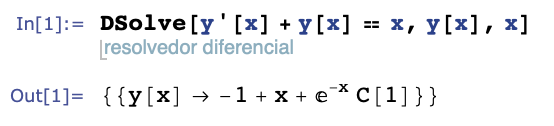
\includegraphics[width=0.5\textwidth]{fig1-35052.png}
 \caption{Uso de la instrucción \textbf{DSolve} durante la resolución de la ecuación diferencial $y'+y=x$.}
 \label{fig1}
 \source{Wolfram-Mathematica 10.4.}
\end{figure}

En su interfaz, el software admite la introducción de la ecuación diferencial en la forma simbólica mostrada en la \Cref{fig1}, como: \textbf{DSolve} $[y'[x]+y[x]=x, y[x], x]$, y devuelve la solución $y(x)$, ${{y[x] \rightarrow -1+x+e^{-x} C[1]}}$, la cual coincide con la propia solución de la ecuación descrita anteriormente en la técnica de la que se siguen los pasos enunciados. 

Sin embargo, observe cómo la fidelidad de los símbolos de entrada y salida en la resolución de la ecuación se desvanece respecto de la notación establecida para estos últimos en los pasos mencionados. Por ejemplo, la notación funcional para $y'(x)$, requiere que la variable independiente se encierre dentro de un corchete $y'[x]$, en letra normal; algo semejante ocurre con la constante de integración dispuesta como $C[1]$. En este sentido, los elementos de la notación que devuelve la interfaz solo se “parecen” a los símbolos vistos durante el desarrollo de la técnica $\tau$ pero no corresponden a la forma utilizada de los signos. Además, la aplicación elegida desde Wolfram-Mathematica no contempla los pasos seguidos para la resolución de la ecuación diferencial, dejando de lado la riqueza conceptual ahí contenida. Esta es la parte más débil del software, puesto que no permite a los alumnos verificar los pasos seguidos para la resolución de la ecuación, devolviendo solamente la solución, lo cual evita que la aplicación contribuya en la adquisición de capacidades por parte del usuario, toda vez que la visibilidad de la matemática es parcializada por el algoritmo que respalda al software.

El desarrollo de capacidades es el objetivo principal que se busca en los cursos de matemáticas del TecNM, por ejemplo, para el curso de EDO, la competencia específica del curso que debe desarrollarse afirma “(El alumno) aplica los métodos de solución de ecuaciones diferenciales ordinarias para resolver problemas que involucran sistemas dinámicos que se presentan en la ingeniería” \cite{tecnologico_nacional_de_mexico_tecnm_ecuaciones_2016}.

En resumen, la fidelidad en la notación usada tanto en el aula como en el software, determina una distancia simbólica y conceptual que lleva a discriminar el uso de Wolfram-Mathematica, al menos para el tema visto. La distancia la establece el desarrollador del software durante el tránsito de símbolos de la matemática escolar a este último. Además, el software solo es útil en el escritorio de la computadora. Lo deseable es que se adaptara al móvil de los estudiantes, puesto que todos cuentan con uno de estos, considerando que la aplicación es orientada a cubrir sus necesidades en el aula. Estas imposibilidades técnicas son comunes en la diversidad de software que se reconoce actualmente. Un caso semejante es la “nube de Geogebra” que precisa del uso de internet para interactuar con la herramienta \cite{salas2018}.

Cabe destacar que el uso de software comercial garantiza la resolución de problemas de la matemática, tanto en el ambiente escolar como en profesiones intermediarias de la ingeniería, así como en el desarrollo de proyectos de investigación que involucran conocimientos de la física-matemática.

El objetivo del escrito es analizar un desarrollo tecnológico app.m, el cual es arropado por la línea de investigación Tecnologías Aplicadas a la Educación (TAE) que pertenece a la Maestría en Sistemas Computacionales del TecNM. Buscamos establecer el grado de fidelidad entre la simbología matemática que devuelve la interfaz de la aplicación, respecto de aquella que describen los estudiantes en sus cuadernos de trabajo.

Estas creaciones forman parte de un proyecto de investigación más amplio que tiene por interés desarrollar ese tipo de aplicaciones para diferentes temas incluidos en los cursos de matemáticas que se enseñan en el TecNM. El objetivo del proyecto es contar con herramientas tecnológicas útiles en el salón de clase, que agilicen la resolución de problemas que se proponen a los estudiantes.

En el escrito se usa como eje transversal la resolución de EDO, no obstante, la diversidad de temas posibles contenidos en los programas de estudio forma parte de un nutrido grupo de proyectos de investigación que se ofrecen a los tesistas.

\section{Marco teórico}
Como norma, el concepto de fidelidad determina las características del software que se requiere utilizar en el salón de clase. Sin embargo, por su versatilidad, atañen aquellas app\footnote{Del ingles, \emph{app}: Application a Computer Program. Aplicación que ayuda a los usuarios a resolver una tarea.} que resuelven problemas de la matemática escolar, distinguidas en \textcite{camachorios2019} como app.m, que en español toma el significado figurado de aplicaciones matemáticas para Android. Es decir, aquellas que se descargan al móvil y se utilizan sobre el mismo, en el entorno del salón de clase, sea virtual o presencial. La versatilidad de este tipo de software refiere cualidades (que denotaremos a continuación con el símbolo $\gamma$) como su capacidad de adaptarse con rapidez y facilidad, tanto al móvil como a los usuarios. Las principales cualidades que se exigen en su construcción han sido problematizadas por \textcite{garcia2020}, son las que se muestran enseguida.

\begin{description}
\item[$\gamma_1$] Que se pueda descargar en el móvil de los estudiantes.
\item[$\gamma_2$] Que no requiera de internet para su uso.
\item[$\gamma_3$] Que el lenguaje simbólico utilizado en la app.m sea fiel respecto al utilizado por
los estudiantes.
\item[$\gamma_4$] Que devuelva los pasos a seguir durante la resolución de problemas.
\item[$\gamma_5$] Que su costo sea nulo.
\end{description}

La cualidad $\gamma_4$ exige utilizar la mejor técnica $\tau$ la cual se desprende conceptualmente de las definiciones desarrolladas por el profesor en el salón de clase. En este rubro se encuentran tres cuestiones fundamentales que llevan a la resolución de problemas por parte de los estudiantes. La primera refiere una actividad, o tarea, \emph{T} que los estudiantes deberán resolver utilizando la técnica $\tau$ dispuesta en la app.m. La técnica se desprende de un teorema o definición, que denotaremos con el símbolo $\theta$, cuya demostración establece el profesor en el pizarrón. 

En el ejemplo referido líneas arriba para la resolución de la ecuación lineal (\ref{eq01}), el profesor, a través de esta última, construye la definición para el factor de integración $\mu(x) = e^{\int P(x)d x}$, que se aprecia en $\tau_2$, el cual organiza la técnica mencionada. De este modo se configura una “unidad de análisis” de la siguiente forma:

% \begin{description}
% \item[$\theta$]: $\begin{aligned}[t]
% \mu(x) = e^{\int P(x)d x} \\
% \tau: \tau_1, \tau_2, \tau_3, \tau_4, \tau_5, \tau_6
% \end{aligned}$
% \item[$T$]: Resolver la ecuación diferencial $y'+ y = x$
% \end{description}

\begin{description}
\item[$\theta$]: $\mu(x) = e^{\int P(x)d x}$
\item[$\tau$]: $\tau_1, \tau_2, \tau_3, \tau_4, \tau_5, \tau_6$
\item[$T$]: Resolver la ecuación diferencial $y'+ y = x$
\end{description}

La unidad de análisis fue definida por \textcite{chevallard2007} como “praxeología” en el marco de la Teoría Antropológica de lo Didáctico (TAD), como la tétrada $[T, \tau, \theta, \Theta]$. En esta última el símbolo $\Theta$ represenra al marco teórico en la que se encuentra la praxeología. Para el caso que nos ocupa ese marco corresponde al Análisis Real. La praxeología involucra una praxis constituida por la técnica $\tau$ y la actividad \emph{T}, así como un \emph{logos} o conocimiento reconocido por $\theta$ y $\Theta$  La unidad de análisis o praxeología, modeliza la actividad en el aula. No obstante, organiza y modela, también, el diseño y desarrollo de aplicaciones app.m orientadas por objetos de la matemática. Desde esta óptica, las exigencias de fidelidad para el desarrollo de las app.m, son vinculadas en la técnica $\tau$, la cual determina un eje central conceptual sobre la interfaz de la aplicación.

El cambio que produce la transición de un conocimiento de la matemática escolar a un ambiente diferente, se reconoce en la TAD como “efecto transpositivo” \cite{chevallard2007, castela2009}. Algo semejante ocurre al transferir símbolos de la matemática, como $y(x)$, en el ejemplo citado, contra aquellos que devuelve \emph{Mathematica}, $y[x]$. Por el ambiente informático al que se mueven estos conocimientos, llamaremos a esa transición “efecto transpositivo informático” (ETI). La verificación de los ETI en el software y app.m, garantiza el nivel de fidelidad de los símbolos dispuestos en la interfaz del software, respecto de aquellos que utilizan los estudiantes en sus cuadernos. Los ETI corresponden a casos particulares de los efectos que determina la “transposición informática” desarrollada por \textcite{balacheff}.

\section{Metodología}
\textcite{santostrigo2018} enfatizan la importancia de integrar diversas tecnologías y recursos digitales en la enseñanza de la matemática. Pero ¿Cuáles son aquellas aplicaciones tecnológicas que por sus características técnicas y didácticas se pueden llevar al aula? Desde el enfoque ETI y las cinco cualidades propuestas por \textcite{garcia2020} como $\gamma_1, \gamma_2, \gamma_3, \gamma_4, \gamma_5$ se analizan enseguida algunas de las app.m más conocidas y utilizadas en el escenario de la matemática escolar. Se incluye también, en el apartado 4, el análisis a la aplicación desarrollada por \textcite{garcia2020}. Algunas de las examinadas se encuentran en GooglePlay y App Store. El procedimiento seguido fue:

\begin{enumerate}[label=(\alph*)]
\item Se realizó una búsqueda en internet para identificar las app.m que resuelven ecuaciones diferenciales ordinarias.
\item De las aplicaciones encontradas se eligieron las que aparecían en forma constante.
\item Se procedió a resolver en cada una el mismo ejercicio para verificar la forma de resolución, las indicaciones mostradas, el resultado y la fidelidad en la técnica utilizada para cada paso mostrado. La EDO por resolver fue: $y'+y=x$
\item Analizamos la facilidad de descarga, el costo, el uso de datos móviles.
\item Respecto a la forma en que muestran el procedimiento y el resultado, nos preguntamos si estos coinciden con el lenguaje y procedimiento utilizados en el aula.
\end{enumerate}

Por su reconocimiento y uso en la comunidad estudiantil de las carreras de ingeniería del TecNM, analizamos ocho aplicaciones (de entre una buena cantidad que se encuentran en la web): la primera es Symbolab, la cual fue elegida por la sencillez en el ingreso de datos y vuelta de resultados, toda vez que cuenta en su interfaz con editor de ecuaciones confiable. Resuelve todo tipo de expresiones matemáticas, como derivadas, integrales, EDO, etc. La segunda es MathDF, esta determina diversos tipos de problemas relacionados con la matemática utilizada en los cursos de los niveles de enseñanza medio superior y superior. La tercera se conoce como WolframAlpha y corresponde a la versión app.m del software Wolfram-Mathematica, comentado líneas arriba. Se encuentra entre las mejores aplicaciones desarrolladas para ser utilizada en el salón de clase. La cuarta es Maple Calculadora, en cuanto a su utilidad, es semejante a WolframAlpha, cuenta con un cuadro de texto y un teclado para ingresar la información.

Una aplicación muy utilizada por los estudiantes en las asignaturas de matemáticas es Photomath, ya que es posible escribir en el cuaderno el problema y escanearlo con la cámara del teléfono móvil, y muestra todos los pasos para alcanzar la solución. La sexta app revisada fue Algemator, la cual utiliza un lápiz virtual para escribir las ecuaciones.  Tanto Photomath como Algemator están disponibles sólo en versión móvil para Android y iPhone.

Otra app analizada fue Sr. Examen, sólo es posible utilizarla en la web, en versión gratuita y el procedimiento es parcialmente semejante al utilizado en el aula, incluye teoría. Por último, se eligió Ecuaciones diferenciales de Ivan Petuhov, disponible en la PlayStore y AppStore la cual tiene la desventaja de que sólo presenta el resultado; para visualizar el procedimiento existe versión de paga. 

\subsection{Análisis de app.m desde los ETI}\label{sec-3.1}
En la \Cref{tab1} hemos dispuesto las características principales de las app.m analizadas desde la perspectiva sugerida. Coincidimos con Leung cuando menciona:

\begin{quote}
La propia experiencia de aprendizaje de los profesores con herramientas digitales es fundamental en la formación de su conocimiento integrado en tecnología. Los profesores deben experimentar por sí mismos, como estudiantes, los potenciales y los peligros de la herramienta digital en el aprendizaje de las matemáticas \cite[p. 6]{leung2017}.
\end{quote}

En tal sentido, solo nos interesamos por las características mencionadas y no estudiamos sus especificaciones técnicas. La mayoría de las aplicaciones se descargan al móvil sin ningún inconveniente. Symbolab utiliza un lenguaje semejante al usado por los estudiantes en sus cuadernos, pero los paréntesis en las funciones son faltos de proporción. En el resto de las aplicaciones la notación para introducir el ejercicio es idéntica a la utilizada en clase. En los casos de Symbolab, WolframAlpha y Maple Calculadora, estas, devuelven en lo inmediato la solución del problema solicitado, pero, para exhibir la totalidad de la técnica, solicitan un cobro adicional. Esto último no ocurre con MathDF, la cual arroja la técnica completa, solo que con métodos diferentes a los que se ven en el salón de clase. Algo semejante ocurre con WolframAlpha, la cual, también, devuelve gráficas relacionadas con los problemas. De entrada, las app.m analizadas son gratuitas, no obstante, en los casos citados es necesario pagar una cuota para obtener el total de los pasos que surgen del proceso de resolución.

\begin{longtable}{p{0.12\textwidth}p{0.12\textwidth}p{0.12\textwidth}p{0.17\textwidth}p{0.15\textwidth}p{0.15\textwidth}}
\caption{Se muestra información relacionada con el uso de diferentes app.m.}
\label{tab1}
\\
\toprule
app.m & $\gamma_1$ & $\gamma_2$ & $\gamma_3$ & $\gamma_4$ & $\gamma_5$\\
\midrule
Symbolab 
& Se descarga fácilmente al móvil y disponible versión web 
& Requiere internet para funcionar
& El lenguaje que devuelve en las soluciones tiene la desventaja de utilizar paréntesis muy grandes en la designación de variables. Por ejemplo, en las funciones trigonométricas.
& Devuelve solamente la solución.
& Para solicitar la totalidad de la técnica $\tau$ es necesario realizar un pago extra y suscribirse.
\\
MathDF
& Se descarga fácilmente al móvil y disponible versión web
& Su uso hace necesario estar conectado a internet.
& El lenguaje que devuelve en las soluciones es semejante al utilizado en clase.
& Exhibe los pasos de resolución, utilizando métodos y técnicas diferentes a las expuestas en clase.
& Gratuita.
\\
Wolfram-Alpha
& Se descarga fácilmente al móvil y disponible versión web
& Su uso hace necesario estar conectado a internet.
& El lenguaje que devuelve en las soluciones es semejante, al utilizado en clase. Muestra diversos procedimientos para la solución en la versión de paga.
& Devuelve solamente la solución. En algunos casos incluye la gráfica.
& Para solicitar la totalidad de la técnica $\tau$ es necesario realizar un pago extra que oscila entre 4.75 y 12 dólares, lo cual depende de la versión elegida. El costo de la versión completa para estudiantes es de 160 dólares. 
\\
Maple Calculadora
& Se descarga fácilmente al móvil. 
No disponible en versión web.
& No requiere internet.
& El lenguaje que devuelve en el resultado es semejante al utilizado en clase.
& Solo devuelve el resultado En algunos casos incluye la gráfica.
& Parcialmente gratuita. Para solicitar la totalidad de la técnica $\tau$ es necesario realizar un pago extra.
\\
Photomath
& Sólo versión móvil.
& Requiere internet para funcionar.
& El lenguaje que devuelve en el resultado y el procedimiento es semejante al utilizado en clase.
& Si muestra el procedimiento. Limitado al tipo de ejercicios que resuelve.
& No tiene costo.
\\
Algemator
& Disponible sólo versión móvil
& Requiere internet para funcionar
& El lenguaje utilizado es muy diferente 
& No muestra el resultado hasta entrar a período de prueba
& Para solicitar la totalidad de la técnica $\tau$ es necesario realizar un pago extra.
\\
Sr. Examen
& Sólo versión web.
& Requiere internet para funcionar.
& Los pasos y el lenguaje utilizado son parcialmente semejantes al del aula.
& Si muestra el procedimiento.
& No tiene costo.
\\
Ecuaciones Diferenciales 
Ivan Petuhov
& Disponible en versión móvil.
& Requiere internet para funcionar.
& El lenguaje que devuelve en el resultado es semejante al utilizado en clase.
& Sólo muestra el resultado.
& Para solicitar la totalidad de la técnica $\tau$ es necesario realizar un pago extra.
\\
\bottomrule
\source{Elaboración propia.}
\end{longtable}

Las aplicaciones observadas son valiosas por la finalidad con la que fueron desarrolladas, cual es su uso en el salón de clase. No obstante, su empleo se debilita respecto a las cinco cualidades sugeridas, siendo el costo extra una limitación. En cuanto a los ETI, ninguna de ellas determina un orden en la técnica $\tau$ que devuelve, comparado con el que se sigue en el salón de clase. Incluso, en casi todas, los métodos y técnicas utilizadas en la resolución difieren significativamente respecto de aquellas aplicadas por maestros y estudiantes.

\section{Desarrollo tecnológico}
\textcite{garcia2020} desarrolló una app.m que permite a los estudiantes y usuarios la resolución de EDO de primer orden: lineales y de Bernoulli. Para ese efecto, partió de las cualidades antes mencionadas como $\gamma_1, \gamma_2, \gamma_3, \gamma_4, \gamma_5$.

El desarrollo del software se fundamentó en un proceso de iteración de varios ciclos: descripción de los requisitos, análisis y diseño, desarrollo, así como, prueba, integración e implementación. Al finalizar cada iteración el desarrollo se puso a prueba ante estudiantes del curso quienes utilizaron la aplicación y en los cuales la autora observó sus apreciaciones y dudas. Un grupo de expertos atendió algunas de las etapas, principalmente la última, quienes probaron y validaron la app.m, proponiendo mejoras y correcciones. El proceso se repitió hasta que se obtuvo un producto satisfactorio para los estudiantes.

Para el desarrollo de la aplicación se utilizó Python, lenguaje interpretado que hace hincapié en una sintaxis que favorezca un código legible. Soporta orientación a objetos, programación imperativa y, en menor medida, programación funcional, usa tipado dinámico y es multiplataforma. Es administrado por la Python Software Foundation. Para programar en Python se utilizó, inicialmente, el ambiente de desarrollo Jupyter de la suite Anaconda y después PyCharm de JetBrains: se realizaban los algoritmos de resolución de ecuaciones diferenciales en este para, posteriormente, llevarse al ambiente de Android Studio 

La aplicación fue diseñada para dispositivos móviles, partiendo del supuesto que los estudiantes del curso de EDO cuentan con uno de estos, toda vez que cumple con las cinco cualidades mencionadas. Para la implementación de la interfaz gráfica, se manejó un \emph{framework} de programación de aplicaciones móviles que se pudiera utilizar en conjunto con Python, en este caso se decidió por Android Studio: un ambiente de desarrollo integrado para aplicaciones en sistema operativo Android, toda vez que la autora tenía conocimientos de este último, incluyendo aquellos de la librería Chaquopy, la cual permitió establecer la comunicación entre Android Studio y Python. De tal forma que el desarrollo, o resolución de las ecuaciones, se llevó a cabo en Python y el diseño de la interfaz de usuario en Android Studio.

\begin{quote}
Python se comunica con Java a través de Chaquopy, todo ello en Android Studio. Java recibe los datos de entrada desde la aplicación y los envía a Python, este realiza el algoritmo y devuelve los resultados a Java, para que finalmente se puedan visualizar los resultados en la aplicación \cite[p. 20]{garcia2020}.
\end{quote}

Java entrega a Python los datos de entrada en un archivo de código llamado “lineales.py”, Java los recibe en una clase citada “DatosGraficaSF.java, y se da la comunicación entre estos en el archivo “EjecutarLineales.java”.

\subsection{Herramientas utilizadas}
Entre las librerías utilizadas, Sympy de Python fue utilizada para matemáticas simbólicas. En tanto, Chaquopy permite que Android Studio y Python puedan comunicarse, su descarga e instalación están automatizadas a través del Gradle en Android Studio. Por su lado, Graphview permite realizar diferentes tipos de gráficas, en este caso para la solución de las ecuaciones diferenciales.

\begin{quote}
Se hizo uso, además, de un lenguaje de composición tipográfica TeX, el cual ayuda a que las ecuaciones, sus pasos de resolución y las soluciones, se puedan visualizar en lenguaje matemático, haciendo uso de LaTeX en Python y de MathJax y KaTeX en Android Studio por medio de Mathview que es una biblioteca de vista de terceros, que ayuda a mostrar la fórmula matemática en las aplicaciones de Android más fácilmente \cite[p. 25]{garcia2020}.
\end{quote}

También, se incorporó una condición de frontera, o bien inicial, para la determinación de la constante c, que arroja la solución general de la EDO. 

\section{Resultados y discusión}
En la \Cref{fig2} se advierte el proceso de cálculo seguido en la app.m para determinar la solución de la EDO tratada a lo largo del escrito. En la imagen a) se distingue la presentación de la pantalla de inicio. Aparece una Bienvenida que informa sobre el uso de la misma. En esta el usuario puede optar por resolver ecuaciones lineales, de Bernoulli, incluso de Cauchy-Euler. En la imagen b) se introducen las funciones en x asociadas a la EDO, es decir, $p_{0}(x), p_{1}(x)$ y $q(x)$ las cuales determinan la forma de la ecuación (\ref{eq01}). Aquí se involucra una condición de frontera, o bien inicial, para el ejemplo fue sugerida $y(0) = 1$. En la imagen c) se obtienen los pasos seguidos para la determinación de la solución de la EDO, que en el artículo seguimos a través de la técnica $\tau$. En la imagen d) se reitera la solución de la ecuación diferencial para la condición de frontera y, en la parte baja, su gráfica en coordenadas rectangulares, en este caso una recta. Algunos resultados se comentan enseguida.

\begin{itemize}
\item Las respuestas analítica e informática que devuelve la interfaz, satisfacen con certeza las cinco cualidades consideradas y no se aprecian ETI que perjudiquen el nivel de fidelidad exigido, lo cual es valioso para una aplicación de este tipo.
\item El uso de LaTex en Python fue la clave para asegurar la fidelidad del lenguaje usado por los estudiantes en su cuaderno respecto del que devuelve la interfaz del móvil. 
\item En lo que se refiere a la resolución de EDO lineales, probamos la app.m para los Ejercicios 2.3 (ecuaciones diferenciales de primer orden) que se proponen en \textcite[p. 62-63]{zill2018}. La aplicación respondió con rapidez y satisfactoriamente a la mayoría. 
\item Además, la app.m es confiable como apoyo alternativo en la resolución de problemas reales, como los propuestos por el mismo autor, Ejercicios 1.3 (Introducción a las ecuaciones diferenciales).
\item El algoritmo diseñado para la Aplicación sigue las actividades de la técnica $\tau$, en la forma desarrollada en el ejemplo líneas arriba, es decir, $\tau: \tau_1, \tau_2, \tau_3, \tau_4, \tau_5, \tau_6$. De modo que despliega en la interfaz cada uno de los pasos que siguen los estudiantes al resolver ese tipo de EDO en su cuaderno.
\item Además, al final del recorrido presenta la gráfica de la solución.
\item Sin embargo, para la resolución de ejercicios, adolece de formas expresivas que permitan introducir en algunas funciones signos y extensiones numéricas. Por ejemplo, la función $e^{x}$ se declara en la interfaz como $exp(x)$ y no da lugar para ingresar el signo negativo ni coeficientes, como en $e^{-2x}$. Algo semejante ocurre con las funciones trigonométricas. 
\item También, en el caso del acceso de la condición de frontera, o inicial, las comillas ahí dispuestas hacen incómodo su ingreso, siendo necesario eliminarlas, lo cual toma algunos segundos. Incluso, en algunas ecuaciones la introducción de la condición hace que la aplicación no responda, lo cual lleva a pensar que la estructura algorítmica cuenta, todavía, con errores de programación.
\item Como se ha mencionado, la aplicación fue desarrollada a través de las cualidades $\gamma_1, \gamma_2, \gamma_3, \gamma_4, \gamma_5$ lo cual favorece su utilidad en el aula en la resolución de EDO. Sin embargo, la aplicación no tiene punto de comparación con la cantidad de problemas que resuelven las app.m analizadas en la sección \ref{sec-3.1}.
\end{itemize}

\begin{figure}[htbp]
 \centering
 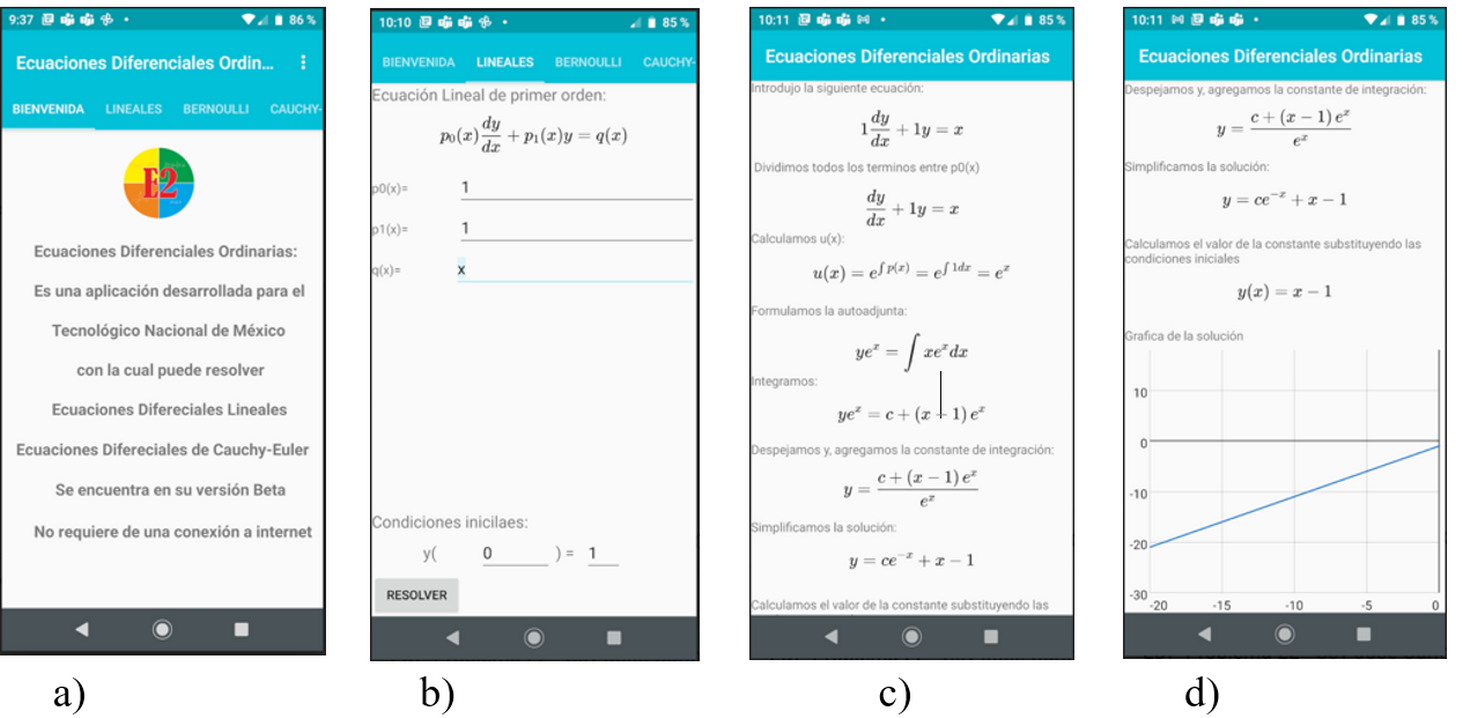
\includegraphics[width=0.95\textwidth]{fig2-35052.png}
 \caption{Imágenes de la app.m que muestran el proceso de cálculo de una EDO en la interfaz del móvil de los estudiantes. La imagen a) exhibe la pantalla inicial; en b) se sugieren los datos de entrada; c) expone los pasos de cálculo seguidos y d) presenta la solución de la EDO, incluyendo su gráfica.}
 \label{fig2}
 \source{Capturas de pantalla desde la aplicación.}
\end{figure}

\section{Conclusiones y desarrollos futuros}
El uso indiscriminado de software por parte de los estudiantes, principalmente aquellos que se encuentran en la web, los lleva a una búsqueda rápida e inmediata de soluciones de ejercicios propuestos como tareas en el aula. Las más de las veces, las aplicaciones resuelven los ejercicios y ofrecen la solución en su interfaz. No obstante, a los estudiantes les cuesta dar una interpretación congruente de los resultados devueltos, por distintas razones. Algunas tienen que ver con métodos de solución diferentes a los vistos en clase, otros con el uso de técnicas matemáticas incompletas e, incluso, la confusión a la que lleva una notación también diferente a la que se utiliza en el cuaderno. Estas ambigüedades se aprecian de una aplicación a otra, sin que en su creación haya una norma que las distinga. Algo semejante ocurre con las soluciones que se ofrecen en YouTube, en las cuales se simplifica la técnica obviando explicaciones y demostraciones como en MateFacil.

El caso analizado en \textcite{garcia2020}, así como otros no menos importantes, como el de \textcite{duarte2020}, en cuya aplicación se obtienen series de Fourier, alientan el desarrollo institucional-escolar de app.m, puesto que las desviaciones ETI del lenguaje matemático entre estas aplicaciones y la notación usada en los cuadernos de los estudiantes es mínima, sin percibirse, en diversos ejercicios, los errores de programación en la versión de la app.m analizada.

Ese estrecho acercamiento de la informática al aula favorece con su inmersión la creatividad del profesor en posibles diseños de situaciones didácticas, en las cuales sea posible involucrar aplicaciones que hagan más atractiva la actividad de enseñanza. La tendencia, en este sentido, lleva al móvil a convertirse en un pequeño laboratorio portátil de matemáticas, de amplia utilidad para los usuarios, lo cual favorece sus propias capacidades. Un posible adiós desde el aula a las Laptop y calculadoras científicas, entre otras herramientas. Aciago, pero afortunado, futuro. 


%%%%%%%%%%%%%%%%%%%%%%%%%%%%%%%%%%%%%%%%%%%%%%%%%%%%%%%%%%%%%%%%%%%%%%%%%%%%%%%%%%%%%%%%%%%%%%%%%%%%%%%%%%%%%%%%%%%%%%%%%%%%%%%%%%%%%%%%%%%%%%%%%%%%%%%%%%%%%%%%%%%%%%%%%%%%%%%%%%%%%%%%%%%%%%%%%%%%%%%%%%


\printbibliography\label{sec-bib}
% if the text is not in Portuguese, it might be necessary to use the code below instead to print the correct ABNT abbreviations [s.n.], [s.l.] 
%\begin{portuguese}
%\printbibliography[title={Bibliography}]
%\end{portuguese}

%full list: conceptualization,datacuration,formalanalysis,funding,investigation,methodology,projadm,resources,software,supervision,validation,visualization,writing,review
\begin{contributors}[sec-contributors]
\authorcontribution{Alberto Camacho Ríos}[conceptualization,writing,investigation,funding]
\authorcontribution{Bertha Ivonne Sánchez Luján}[validation,formalanalysis,review,investigation,software]
\authorcontribution{Marisela Caldera-Franco}[investigation,methodology,software]
\end{contributors}


\end{document}
